\chapter{Outil mis à disposition du service de détection des fraudes}
\label{chap:outil-operationnel}

Le présent chapitre traite du second outil créé à l'aide de l'Intelligence Artificielle.

Ce dernier se présente sous forme d'une interface utilisateur proposant trois fonctionnalités :

\begin{enumerate}
    \item Évaluer un ou plusieurs nouveaux sinistres : l'utilisateur dépose un fichier contenant des informations sinistres pour estimer, pour chaque dossier, sa probabilité de fraude intrinsèque ;
    \item Renseigner le résultat de fraude de sinistres testés précédemment : cela permettra d'enrichir la base de données utilisée pour la construction du modèle dans l'outil précédent ;
    \item Consulter le bilan annuel de fraude : l'utilisateur peut lire les analyses sur les fraudes de l'année (montant économisé, rapport sur les mécanismes de fraudes récurrents, etc.).
\end{enumerate}

Ces différentes fonctionnalités seront décrites en détail dans les paragraphes suivants.

\begin{figure}[H]
    \centering
    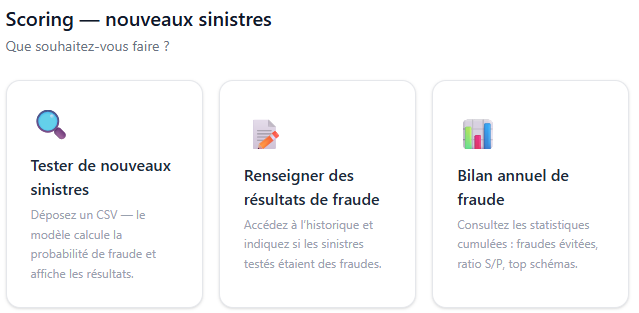
\includegraphics[width=0.9\textwidth]{images/chapitre6/interactif.png}
    \caption{Écran interactif d'accueil du second outil}
    \label{fig:ecran-accueil-outil2}
\end{figure}

% --------------------------------------------------------------
\section{Utilisation pratique de l'outil}
% --------------------------------------------------------------

L'outil mis à disposition du service de détection des fraudes constitue la traduction opérationnelle du modèle de détection des fraudes développé en amont. Il s'inscrit dans une logique d'\textbf{aide à la décision fondée sur une estimation probabiliste du risque de fraude}, permettant d'orienter de manière cohérente et homogène les actions de contrôle sur les sinistres.

En amont de son utilisation, les seuils de décision sont définis par l'actuaire en charge du modèle, puis transmis aux gestionnaires sinistres pour paramétrage dans l'outil. Ces seuils permettent de segmenter l'espace des probabilités en différentes zones de risque.

À ce stade, on retient à titre illustratif le dernier modèle (Gradient \textit{Boosting}) et les seuils suivants :

\begin{itemize}[label = $\bullet$]
    \item $Seuil_{\inf} = Seuil_{optimal} - 10~\%$
    \item $Seuil_{\sup} = Seuil_{optimal} + 10~\%$
\end{itemize}

Ce qui crée naturellement les trois zones :

\begin{itemize}[label = $\bullet$]
    \item \textcolor{vert}{Une zone de faible risque (verte) : $[\,0 \, ; \, Seuil_{\inf}[$}
    \item \textcolor{orange}{Une zone de risque intermédiaire (orange) : $[\,Seuil_{\inf} \, ; \, Seuil_{\sup}[$}
    \item \textcolor{rouge}{Une zone de risque élevé (rouge) : $[\,Seuil_{\sup} \, ; 100~\%]$}
\end{itemize}

Ces seuils traduisent un arbitrage actuariel entre le \textbf{coût des investigations} (notamment en termes de ressources mobilisées et de délais de gestion) et le \textbf{gain attendu lié à la détection de fraude}, en tenant compte des taux de faux positifs et de faux négatifs.

Lorsque l'utilisateur clique sur « tester de nouveaux sinistres », l'outil demande ensuite à l'utilisateur de renseigner les caractéristiques d'un ou plusieurs sinistres pour lancer l'analyse. Cette intégration peut s'effectuer de deux manières : soit de façon industrielle par le dépôt d'un fichier standardisé, soit de manière unitaire via un formulaire de saisie manuelle (cf. illustration ci-dessous).

\begin{figure}[H]
    \centering
    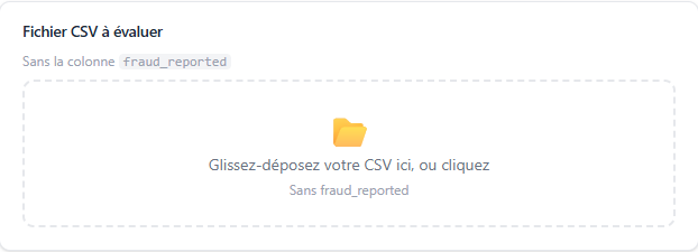
\includegraphics[width=0.9\textwidth]{images/chapitre6/deposer_csv.png}
\end{figure}

Ces flux d'entrée reprennent exactement les mêmes variables explicatives que notre base de modélisation (franchise, âge, profession, type d'incident, montants, etc.), mais sans intégrer la colonne cible de fraude avérée (\textit{fraud\_reported}).

\begin{figure}[H]
    \centering
    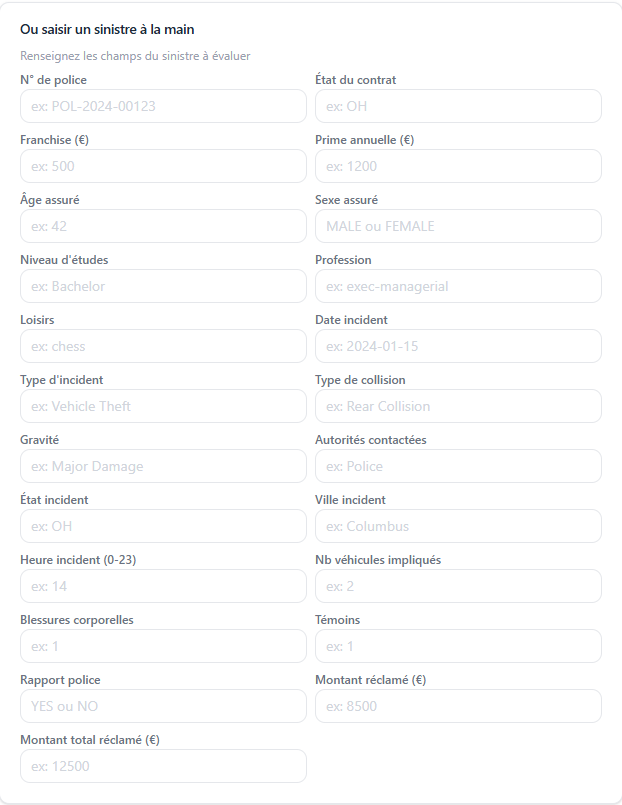
\includegraphics[width=0.7\textwidth]{images/chapitre6/saisie_manuelle.png}
    \caption{Saisie manuelle des informations sinistre pour évaluation de la probabilité de fraude}
    \label{fig:saisie-manuelle}
\end{figure}

Sur la base des informations sinistre renseignés, le modèle calcule une \textbf{probabilité de fraude en appliquant le modèle retenu dans l'outil de modélisation de la fraude.}

Cette probabilité constitue une mesure synthétique du risque, intégrant l'ensemble des signaux de fraude identifiés lors de la phase de modélisation.

La décision opérationnelle repose alors sur la \textbf{comparaison de cette probabilité aux seuils définis dans l'outil précédent (enregistrés en paramètres)}. Chaque sinistre est ainsi affecté à une classe de risque, à laquelle est associée une stratégie de gestion différenciée :

\begin{itemize}[label = $\bullet$]
    \item Absence d'investigation pour les niveaux faibles ;
    \item Contrôles ciblés pour les niveaux intermédiaires ;
    \item Et investigations approfondies pour les niveaux élevés.
\end{itemize}

Ce dispositif permet d'optimiser la \textbf{fonction de coût globale} du processus de détection, en concentrant les efforts sur les dossiers présentant le meilleur ratio entre probabilité de fraude et coût d'investigation.

À titre d'illustration, sur un échantillon test de 500 sinistres, l'outil réalise un filtrage puissant en isolant immédiatement 474 dossiers en zone verte (ne nécessitant aucune investigation humaine), 21 dossiers en zone orange (à surveiller ou contrôler superficiellement) et seulement 5 dossiers en zone rouge (faisant l'objet d'une alerte prioritaire).

\begin{figure}[H]
    \centering
    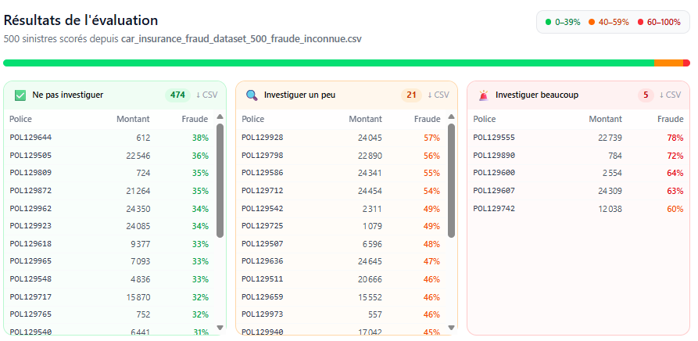
\includegraphics[width=0.9\textwidth]{images/chapitre6/tableau_proba.png}
    \caption{Probabilité en sortie de l'outil}
    \label{fig:tableau-proba}
\end{figure}

Ainsi, l'outil s'inscrit dans une démarche actuarielle classique de \textbf{segmentation du risque et de prise de décision sous contrainte}, en transformant une estimation probabiliste issue du modèle en règles de gestion opérationnelles directement exploitables par les équipes métiers.

L'utilisation d'un tel outil présente plusieurs avantages majeurs dans le cadre de la détection de fraude, tant d'un point de vue actuariel qu'opérationnel. En premier lieu, il permet de \textbf{standardiser l'évaluation du risque de fraude} en s'appuyant sur un modèle statistique commun, appliqué de manière homogène à l'ensemble des sinistres. Cette standardisation réduit significativement les \textbf{variabilités de traitement entre gestionnaires}, liées à l'expérience, à la subjectivité ou à la sensibilité individuelle au risque, et garantit une plus grande cohérence dans les décisions prises.

En outre, l'outil favorise une \textbf{objectivation du processus de décision} en reposant sur une estimation probabiliste issue de données historiques. Il limite ainsi les biais cognitifs (sur- ou sous-estimation du risque, effet d'ancrage, etc.) et permet d'inscrire la détection de fraude dans une démarche plus rigoureuse et traçable. Chaque décision d'investigation peut être justifiée par un niveau de risque mesuré, ce qui améliore la \textbf{transparence et l'auditabilité} des pratiques.

Par ailleurs, en segmentant les sinistres selon leur niveau de risque, l'outil permet une \textbf{allocation optimale des ressources d'investigation}. Les dossiers les plus susceptibles d'être frauduleux sont priorisés, ce qui augmente l'efficacité globale du dispositif tout en maîtrisant les coûts liés aux contrôles. Cette approche s'inscrit dans une logique actuarielle d'optimisation du couple \textbf{coût de détection / gain attendu}, en maximisant la rentabilité des actions de lutte contre la fraude.

Enfin, cet outil constitue un levier d'\textbf{harmonisation et de pilotage} à l'échelle du portefeuille. Il permet de suivre la performance du dispositif (taux de fraude détectée, taux de transformation des contrôles, etc.), d'ajuster les seuils de décision en fonction des résultats observés, et d'assurer une meilleure comparabilité dans le temps. Il contribue ainsi à structurer la fonction fraude autour d'indicateurs quantitatifs et d'une approche pilotée par la donnée.

% --------------------------------------------------------------
\section{Un outil permettant l'enrichissement du modèle en continu}
% --------------------------------------------------------------

Dans une logique d'amélioration continue, l'outil intègre un mécanisme de boucle de retour d'information (\textit{feedback loop}) permettant d'enrichir progressivement la base de données d'apprentissage. Ce mécanisme repose sur une base "historique" (ensemble des sinistres renseignés dans l'outil afin d'obtenir une probabilité de fraude), dans laquelle sont automatiquement archivés l'ensemble des sinistres soumis à l'outil, accompagnés de la probabilité de fraude qui leur a été attribuée.

\begin{figure}[H]
    \centering
    
\includegraphics[width=0.55\textwidth]{images/chapitre6/schema_macro.png}
    \caption{Schéma macro du mécanisme d'enrichissement de la base de données}
    \label{schéma_macro}
\end{figure}

Comme l'illustre le schéma ci-dessus, lorsque l'utilisateur soumet un nouveau sinistre pour en estimer la probabilité de fraude, le dossier scoré rejoint la base historique. À ce stade, cette base ne contient toutefois pas encore l'information la plus précieuse pour le modèle : l'issue réelle du dossier. Savoir si un sinistre s'est effectivement révélé frauduleux n'est en effet connu qu'à l'issue de son instruction, souvent plusieurs semaines, voire plusieurs mois, après la déclaration. C'est ce constat qui structure la logique d'enrichissement retenue.

Plutôt que de demander au gestionnaire de statuer immédiatement sur une fraude qu'il ne peut encore confirmer, l'outil lui permet de revenir à tout moment dans la base historique pour y renseigner le statut final d'un ou plusieurs sinistres (fraude avérée ou non). \textbf{Cette dissociation entre le moment du \textit{scoring} et celui de la qualification reflète fidèlement la réalité opérationnelle de la gestion des sinistres, où le dénouement d'un dossier est par nature différé.}

\begin{figure}[H]
    \centering
    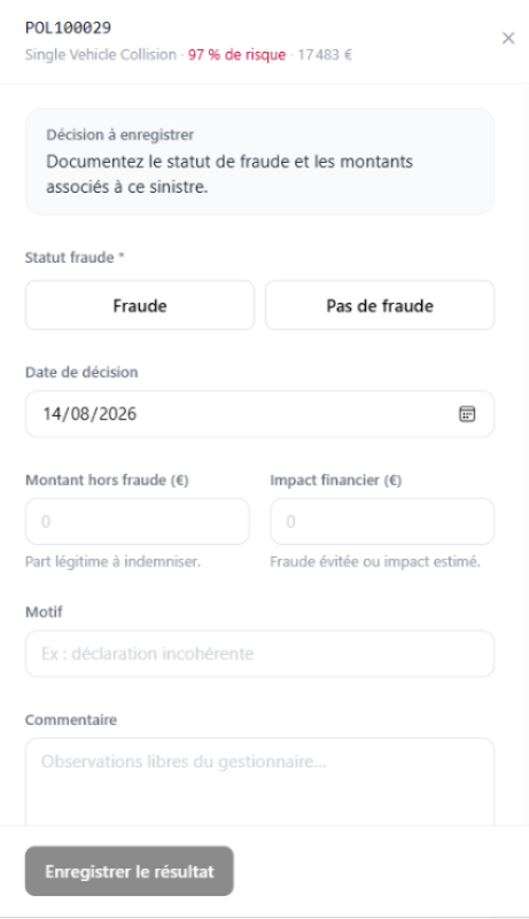
\includegraphics[width=0.55\textwidth]{images/chapitre6/renseignement_sinistre.png}
    \caption{Fiche de renseignement d'un sinistre à l'issue d'une investigation}
    \label{fig:renseignement-sinistre}
\end{figure}

Une fois cette issue renseignée, le sinistre concerné dispose d'un couple complet d'informations : ses caractéristiques d'entrée d'une part, et sa variable cible de fraude (\textit{fraud\_reported}) d'autre part. Il devient alors une observation exploitable pour l'apprentissage, au même titre que les données ayant servi à la construction initiale du modèle. C'est bien un statut binaire, et non une probabilité, qui alimente ainsi la base : un sinistre confirmé comme frauduleux après investigation est enregistré à 1, tandis qu'un sinistre investigué mais jugé finalement légitime est enregistré à 0. Le modèle ne se réentraîne donc que sur des cas dont l'issue est avérée, et non sur de simples suspicions, ce qui garantit la fiabilité de son apprentissage au fil du temps.

A noter que \textbf{l'enrichissement de la base de données ne modifie pas le modèle de façon instantanée}. En effet le réentraînement s'effectue en repassant par le module de construction (Module 1), qui refait tourner le modèle sur la base augmentée des nouvelles observations qualifiées. En pratique, cette opération est à mener à intervalles de temps réguliers (, typiquement une fois par an), afin d'intégrer un volume significatif de nouveaux cas tout en garantissant la stabilité du dispositif entre deux mises à jour.

Cette approche présente plusieurs intérêts sur le plan actuariel. D'abord, elle permet d'augmenter la taille et la représentativité de la base d'apprentissage, en y intégrant des cas récents qui reflètent l'évolution des comportements frauduleux et des méthodes de fraude utilisées. Elle contribue ainsi à réduire le décalage entre les données historiques initiales et la réalité opérationnelle, dans un contexte où les schémas de fraude évoluent rapidement.

Ensuite, ces nouvelles observations permettent un recalibrage et une réestimation réguliers du modèle : actualisation des paramètres, amélioration de la capacité de discrimination et, le cas échéant, réajustement de la pondération des variables. L'objectif est de maintenir dans le temps une performance prédictive stable, mesurée à l'aide d'indicateurs tels que l'AUC, le Gini ou les courbes de gains, et de surveiller l'absence de dérive du modèle (notamment via le \textbf{Population Stability Index}).

Enfin, l'intégration systématique des issues réelles permet de mieux maîtriser certains biais inhérents aux dispositifs de détection, en particulier le biais de sélection lié aux dossiers investigués. En alimentant la base avec les décisions finales issues de l'ensemble des sinistres traités (et non des seuls dossiers ayant fait l'objet d'une alerte) le modèle gagne en robustesse et en cohérence.

Ainsi, l'outil ne se limite pas à une utilisation statique du modèle : il s'inscrit dans une démarche dynamique de modélisation itérative, où chaque sinistre qualifié vient affiner la connaissance du risque et améliorer la pertinence du dispositif de détection.

% --------------------------------------------------------------
\section{Rapport annuel de détection de fraude}
% --------------------------------------------------------------

Au-delà du \textit{scoring} individuel des sinistres, l'outil intègre \textbf{une fonctionnalité de pilotage} offrant une vision agrégée de la performance du dispositif sur une période donnée (paramétrable mais dans les faits, mensuelle ou annuelle). Lancé annuellement, il constitue la synthèse cumulative de l'activité de détection de fraudes : il s'appuie sur l'ensemble des sinistres testés dans l'outil pour obtention de score de fraude et les résultats des investigations renseignés. Ainsi, il permet de ressortir des indicateurs de volume (sur les dossiers traités) mais également économiques (fraude évitée en montant).

Cette vue de synthèse répond à un besoin actuariel essentiel : ne pas se limiter à une utilisation opérationnelle au fil de l'eau, mais disposer d'indicateurs consolidés permettant d'évaluer et de justifier l'utilisation de l'outil et d'ajuster le dispositif mis en place dans le temps.

\begin{figure}[H]
    \centering
    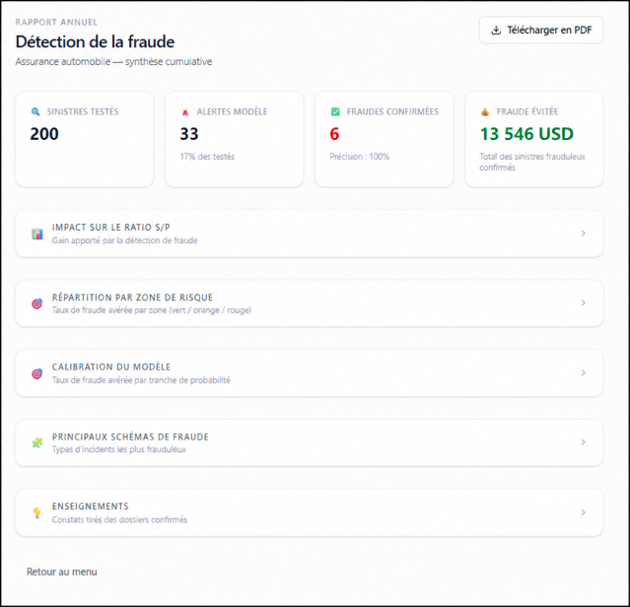
\includegraphics[width=0.85\textwidth]{images/chapitre6/rapport_annuel.png}
    \caption{Extrait du rapport annuel de la détection de fraude}
    \label{fig:rapport-annuel}
\end{figure}

\underline{Dans notre outil, différents indicateurs ont été mis en place} :

\begin{enumerate}

    \item Les premiers indicateurs portent sur le \textbf{volume et la détection} : nombre de sinistres testés, nombre d'alertes générées par le modèle et nombre de fraudes effectivement confirmées après investigation. Leur mise en regard permet d'apprécier la charge de travail générée par l'outil et le taux de concrétisation des alertes.

    \item Viennent ensuite les indicateurs \textbf{financiers}, au cœur de l'enjeu actuariel. Le montant de fraude évitée agrège les sinistres frauduleux confirmés qui n'ont pas donné lieu à indemnisation grâce à l'outil. Pour compléter cet indicateur, un KPI important est également calculé : l'impact sur le \textbf{ratio Sinistres / Primes (S/P)} de la détection de fraude qui traduit directement le gain apporté par la détection sur l'équilibre technique du portefeuille. En effet, en écartant une partie de la charge frauduleuse, l'outil améliore mécaniquement ce ratio. Cet indicateur fait le lien avec l'analyse développée au chapitre~\ref{chap:contexte} : là où nous avions modélisé la surprime supportée par les assurés honnêtes par la relation $\Pi_{\text{chargée}} = \frac{\Pi_{\text{pure}}}{1 - \alpha}$, le rapport annuel permet de quantifier \textit{a posteriori} la part de charge frauduleuse $\alpha$ effectivement récupérée, et donc l'effet réel de l'outil sur la tarification.

    \item Le rapport suit également la \textbf{qualité opérationnelle} du dispositif. La précision de l'outil mesure, parmi les alertes confirmées, la proportion de véritables fraudes, indicateur clé pour éviter de mobiliser inutilement les équipes d'investigation sur des faux positifs. La répartition des sinistres par zone de risque (verte, orange, rouge) permet quant à elle de visualiser la distribution du portefeuille et d'ajuster les seuils $Seuil_{\inf}$ et $Seuil_{\sup}$ si nécessaire.

    \item Enfin, deux indicateurs relèvent d'une logique d'\textbf{intelligence fraude} plus avancée. L'identification des réseaux, en repérant les sinistres impliquant plusieurs véhicules, signale une suspicion de fraude organisée, distincte de la fraude opportuniste. La détection de nouvelles tendances met en évidence l'émergence de schémas de fraude inédits, permettant d'anticiper l'évolution des comportements frauduleux.

\end{enumerate}

L'ensemble se synthétise dans une mesure du \textbf{retour sur investissement (ROI) de l'outil}, rapprochant le gain généré (fraude évitée) du coût de mise en œuvre et d'exploitation du dispositif. Cet indicateur répond directement à la problématique de rentabilité posée en introduction : il démontre que l'automatisation de la détection, en abaissant le coût marginal de contrôle, rend rentable l'analyse de l'ensemble des sinistres, y compris ceux de faible montant jusque-là trop coûteux à investiguer manuellement.

Ce rapport peut par ailleurs être exporté au format PDF, offrant un livrable synthétique directement transmissible à la Direction Technique, au service anti-fraude ou aux instances de gouvernance. Cette possibilité d'extraction facilite le \textit{reporting} périodique et la traçabilité des résultats, en cohérence avec les exigences de documentation évoquées dans le cadre de gouvernance de l'outil (cf.~section~\ref{sec:gouvernance}).

Ainsi, le rapport annuel transforme l'outil de détection en véritable instrument de pilotage actuariel. Il ne se contente pas de traiter les sinistres individuellement, mais fournit une lecture consolidée et chiffrée de la performance du dispositif, permettant de justifier son maintien, d'en ajuster les paramètres et d'en mesurer l'impact réel sur l'équilibre technique du portefeuille.

% --------------------------------------------------------------
\section{Dynamisme de l'outil mis en place}
% --------------------------------------------------------------

Le modèle développé présente un caractère dynamique et évolutif, essentiel dans un environnement assurantiel en constante mutation. Il ne s'agit pas d'un dispositif figé : la plupart des choix effectués tout au long de ce mémoire constituent des hypothèses de travail, retenues pour les besoins de l'illustration, mais paramétrables et substituables sans refonte de l'outil. Le tableau ci-dessous récapitule ces principaux choix de conception et les alternatives envisageables pour chacun.

\begin{table}[H]
    \centering
    \footnotesize
    \renewcommand{\arraystretch}{1.4}
    \begin{tabularx}{\textwidth}{|>{\raggedright\arraybackslash}p{3.2cm}|>{\raggedright\arraybackslash}X|>{\raggedright\arraybackslash}X|}
        \hline
        \rowcolor{accenture}
        \textcolor{white}{\textbf{Élément de l'outil}} & \textcolor{white}{\textbf{Choix retenu dans ce mémoire}} & \textcolor{white}{\textbf{Alternatives / paramétrage possible}} \\
        \hline
        Variables d'entrée & 53 variables (24 variables source + 29 ajoutées pour enrichissement) & Nombre et nature libres : l'outil s'adapte à tout jeu de variables, avec ou sans enrichissement \\
        \hline
        Enrichissement de la base & 29 variables simulées (historique, réparateur, tiers, véhicule, comportement déclaratif, géo-temporel) & Enrichissement facultatif et extensible ; d'autres axes peuvent être ajoutés selon les données réellement disponibles chez l'assureur \\
        \hline
        Modèles de détection & 3 modèles (\textit{scoring} en points, arbre de décision, Gradient \textit{Boosting}) & Architecture agnostique : tout autre modèle de classification (régression logistique, forêt aléatoire, réseau de neurones\ldots) peut être branché \\
        \hline
        Partitionnement train/test & 80 / 20, stratifié sur la cible & Ratio librement modifiable ; validation croisée déjà intégrée sur la partie apprentissage \\
        \hline
        Seuil de décision & Seuil optimal via l'indice de Youden & Réglable manuellement selon l'arbitrage précision/rappel souhaité \\
        \hline
        Zones d'investigation & Bande de $\pm 10~\%$ autour du seuil optimal (3 zones : verte / orange / rouge) & Largeur et nombre de zones paramétrables selon l'appétence au risque et la capacité d'investigation \\
        \hline
        Gestion des valeurs manquantes & Contrôle bloquant (saisie obligatoire d'une valeur) & Imputation automatique possible (moyenne, médiane, modalité la plus fréquente) \\
        \hline
        KPI du rapport de suivi & Fraude évitée, taux d'alertes, impact sur le ratio S/P, ROI & Indicateurs ajoutables ou modifiables selon les besoins de pilotage du management \\
        \hline
        Réentraînement & Boucle continue alimentée par les issues d'investigation & Fréquence de recalibrage paramétrable (au fil de l'eau, périodique\ldots) \\
        \hline
    \end{tabularx}
    \caption{Synthèse des choix retenus et des alternatives de paramétrage de l'outil}
    \label{tab:synthese-choix-outil}
\end{table}

Cette flexibilité constitue un atout majeur pour accompagner les évolutions réglementaires, tarifaires ou opérationnelles des assureurs. Par exemple, l'introduction de nouvelles modalités dans les classes de véhicules (liée à des changements de classification, à l'émergence de nouveaux types de motorisation ou à des ajustements tarifaires) peut être directement intégrée : le modèle réapprend alors les relations entre ces nouvelles modalités et le risque de fraude, sans nécessiter une refonte complète de l'outil.

Ainsi, le modèle s'inscrit dans une logique \textbf{d'amélioration continue}, permettant de maintenir sa pertinence dans le temps. Cette capacité d'adaptation garantit une meilleure prise en compte des évolutions du portefeuille, des comportements frauduleux et du cadre réglementaire, tout en assurant une cohérence avec les pratiques métiers et les politiques de souscription de l'assureur.